\section{Consuntivo}
		In questa sezione verranno riportati il consultivo per le varie fasi di lavoro, considerando le ore sostenute da ogni componente per ruolo. Il bilancio potrà essere:
		\begin{itemize}
			\item \textbf{positivo:} se sono state necessarie meno ore rispetto a quelle preventivate;	 
			\item \textbf{paritario:} se le ore preventivate rispettano quelle effettive;	 
			\item \textbf{negativo:} se sono state necessarie più ore rispetto a quelle preventivate.
		\end{itemize}
	\subsection{Fase di Analisi}
		Le ore di lavoro svolto in questa fase sono di solo investimento e destinate all'apprendimento personale. Di conseguenza queste ore non sono rendicontate. 
		\subsubsection{Prospetto orario}
			Nella tabella in seguito viene illustrato il cambiamento nel numero d'ore di ogni persona, per ogni ruolo ricoperto:
			
			\rowcolors{2}{white}{lightest-grayest}
			\begin{longtable}{|c|c|c|c|c|c|c|c}
				\hline
				\rowcolor{lighter-grayer}
				\textbf{Nome} & \textbf{Re} & \textbf{Am} & \textbf{An} & \textbf{Pg}  & \textbf{Pr}   & \textbf{Ve} & \textbf{Totale} \\
				\hline
				\endfirsthead
				
				\hline
				Giuseppe Vito Bitetti 		& 0 & 8(-1) & 10(+1) & 0 & 0 & 12 & 30\\
				\hline
				\hline
				Lorenzo Dei Negri			 & 6(-2) & 0 & 14(+1) & 0 & 0 & 10(+1) & 30\\
				\hline
				\hline
				Nicolò Frison 					& 0 & 8(-2) & 9(+1) & 0 & 0 & 13(+1) & 30\\
				\hline
				\hline
				Fouad Mouad 				& 0 & 7 & 11 & 0 & 0 & 12 & 30\\
				\hline
				\hline
				Mariano Sciacco 			& 8 & 0 & 12 & 0 & 0 & 10 & 30\\
				\hline
				\hline
				Alessandro Tommasin    & 9(-2) & 0 & 12(+2) & 0 & 0 & 9 & 30\\
				\hline
				\hline
				Giovanni Vidotto 			& 0 & 6(-1) & 9(+1) & 0 & 0 & 15 & 30\\
				\hline 
				\caption{Tabella contenente il prospetto orario preventivato per la fase di analisi}
			\end{longtable}
			\pagebreak	
			
			La tabella può essere riassunta nel seguente istogramma:
			
			\begin{figure}[H]
				\centering
				\includegraphics[width=0.8\linewidth]{./images/analisiCons1.png}
				\caption{Grafico consultivo ore/ruolo componenti nella fase di Analisi}
				\label{fig:consultivo grafico suddivione ruoli fase Analisi}
			\end{figure}
			
		\subsubsection{Prospetto economico}
			In base al prospetto orario, quello economico sarà il seguente: 
			
			\rowcolors{2}{white}{lightest-grayest}
			\begin{longtable}{|c|c|c|c|c|c|c|c}
				\hline
				\rowcolor{lighter-grayer}
				\textbf{Ruolo} & \textbf{Ore} & \textbf{Costo in €} \\
				\hline
				\endfirsthead
				
				\hline
				Responsabile & 23(-4) & 690,00 (-120,00)\\
				\hline
				\hline
				Amministratore & 29(-4) & 580,00 (-80,00)\\
				\hline
				\hline
				Analista & 77(+6) & 1.925,00(+150,00)\\
				\hline
				\hline
				Progettista & - & -\\
				\hline
				\hline
				Programmatore & - & -\\
				\hline
				\hline
				Verificatore & 81(+2) & 1.215,00(+30,00)\\
				\hline
				\textbf{Totale} & 210 & 4.410,00(-20,00)\\
				\hline
				\caption{Tabella contenente il prospetto economico in riferimento al prospetto orario nella tabella 17}
			\end{longtable}
			\pagebreak
			
			La tabella può essere riassunta nel seguente areogramma:
			\begin{figure}[H]
				\centering
				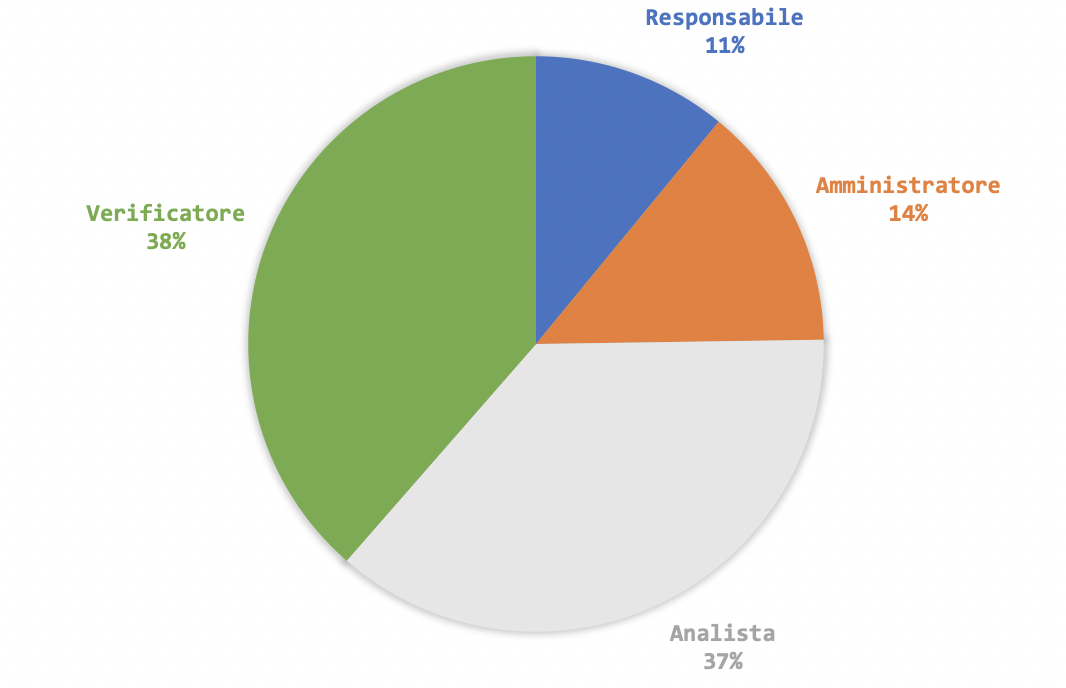
\includegraphics[width=0.8\linewidth]{./images/analisiCons2.png}
				\caption{Grafico percentuale ore/ruolo nella fase di Analisi dei requisiti}
				\label{fig:grafico costi ruolo fase Analisi}
			\end{figure}
		
		\subsubsection{Conclusioni}
			In questa fase il gruppo ha investito il numero di ore che erano state preventivate. È stato necessario però svolgere alcuni cambiamenti nella suddivisione oraria per ruolo, in particolare:
			\begin{itemize}
				\item \textbf{Responsabile:} sono state impiegate meno ore rispetto a quelle preventivate in quanto nella pianificazione del lavoro e nella stesura del Piano di Progetto sono state riscontrate meno difficoltà del previsto;	 
				\item \textbf{Amministratore:} dal momento che i software per la gestione del progetto sono stati individuati e configurati fin da subito e che i documenti sono stati ben strutturati in poco tempo, anche in questo caso sono state impiegate meno ore rispetto a quelle preventivate;	 
				\item \textbf{Analista:} per questo ruolo è stato necessario spendere qualche ora in più in quanto alcuni requisiti, per una corretta comprensione, hanno richiesto una delucidazione esterna con i proponenti del progetto, avvenuta con alcune difficoltà di comunicazione;
				\item \textbf{Verificatore:} poiché alcuni requisiti sono stati individuati tardivamente e di conseguenza per l'aggiunta di contenuti nel documento di Analisi dei Requisiti è stato necessario usufruire di qualche ora in più per controllare nuovamente il documento.
			\end{itemize}
			Alla luce dei cambiamenti effettuati il risultato è che il gruppo ha risparmiato 20,00 € investendo le stesse ore preventivate.
		
		\subsection{Preventivo a finire}
			Trattandosi del primo periodo non rendicontato, non risulta necessario attuare alcuna contromisura nè dal punto di vista del monte ore totale, nè dal punto di vista del preventivo economico; soprattutto considerando che non si è verificato alcun sforamento del budget preventivato.
			
			% Di seguito il preventivo a finire:
			% \rowcolors{2}{white}{lightest-grayest}
			% \begin{longtable}{|c|c|c|c|c|c|c|c}
			% 	\hline
			% 	\rowcolor{lighter-grayer}
			% 	\textbf{Fase} & \textbf{Preventivo in €} & \textbf{Consultivo in €} \\
			% 	\hline
			%	\endfirsthead
			% 	
			% 	\hline
			% 	Analisi & 4.410,00 & 4.390,00\\
			% 	\hline
			% 	\hline
			% 	\textbf{Totale rendicontato} & 13.806,00 & 13.806,00\\
			% 	\hline
			% 	\hline
			% 	\textbf{Totale} & 18.966,00 & 18.966,00\\
			% 	\hline
			% 	\caption{Tabella contenente il preventivo a finire}
			% \end{longtable}
			
			
			